%%% argomento ripreso nel giugno 2022. Qui ci sono le aggiunte.
%%%% questo file dovrebbe sostituire il file giugno21B.tex


%% file utili:
%% contoTrePuntiAllineati.sage

%%%%%%%%%%% buona parte dei
%%%%%%%%%%% file relativi si trovano in directory casoV
%%%%%%%%%%% delta2Properties.sage contiene la dim che delta2=0 da' 3 allin
%%%%%%%%%%% basicConfiguration.sage serve per provare che (6) e (7) non
%%%%%%%%%%% esistono.
%%%%%%%%%%% configurationN5.sage serve a provare che (4) non esiste e
%%%%%%%%%%% invece (5) esiste.
%%%%%%%%%%% delta1_delta1_non_vale.sage prova che due delta1 non vale.
%%%%%%%%%%% configurationN8.sage contiene i conti per il caso (8).


%%%%%%%%%%%%% Dare un'occhiata al file risp19lug


\documentclass{amsart}

\usepackage{amsthm}
\usepackage{amsmath}
\usepackage{graphicx}
%%%%%\usepackage{mathrsfs}  %% \mathscr{A}...
\usepackage{amssymb}
\setlength{\parindent}{.4 in}
\setlength{\textwidth}{5.8 in}
\setlength{\topmargin} {-.1 in}
\setlength{\evensidemargin}{0 in}

\theoremstyle{plain}
\newtheorem{theorem}{Theorem}
\newtheorem{lem}[theorem]{Lemma}
\newtheorem{prop}[theorem]{Proposition}
\newtheorem{cor}[theorem]{Corollary}
\newtheorem{lemma}[theorem]{Lemma}
\newtheorem{rmk}[theorem]{Remark}

\theoremstyle{definition}
\newtheorem{definition}[theorem]{Definition}
\newtheorem{example}[theorem]{Example}

\newcommand{\N}{\mathbb{N}}
\newcommand{\Z}{\mathbb{Z}}
\newcommand{\Q}{\mathbb{Q}}
\newcommand{\R}{\mathbb{R}}
\newcommand{\C}{\mathbb{C}}
\newcommand{\p}{\mathbb{P}}
\newcommand{\sP}{\mathcal{P}}
\newcommand{\sL}{\mathcal{L}}
\newcommand{\sU}{\mathcal{U}}
\newcommand{\sD}{\mathcal{D}}
\newcommand{\sT}{\mathcal{T}}
\newcommand{\sN}{\mathcal{N}}

\newcommand{\de}{\partial}
\newcommand{\codim}{\mathrm{codim}}

\newcommand{\oo}{\mathcal{O}}
\newcommand{\Bl}{\mathrm{Bl}}

\newcommand{\SO}{\operatorname{SO}}
\newcommand{\Eig}{\operatorname{Eig}}
\newcommand{\polq }{{\rm Pol}_Q}
\newcommand{\comment}[1]{}



\newcommand{\scl}[2]{\langle #1, #2 \rangle}
\title{Ternary tensors with an aligned triple of eigenpoints}
\author{}
\date{}
\begin{document}

\maketitle
\begin{abstract}
Abstract
\end{abstract}

\section{Introduction}
\section{Three aligned eigenpoints}
We recall that given a homogeneous form $f\in K[x,y,z]_d$ the eigenscheme $E(f)$ of $f$ is the determinantal scheme defined by the $2\times 2 $ minors of the matrix
%
\begin{equation} 
\label{eq:def_matrix}
    \begin{pmatrix}
    x & y & z \\
    \de_x f & \de_y f & \de_z f
    \end{pmatrix}.
\end{equation}
%   
\begin{lem}
If $E(f)$ is zero-dimensional, then
no degree six subscheme of $E(f)$ lies on a conic.
\end{lem}
\begin{proof}
See \cite[Lemma~9.1]{OS1} for the reduced case. The proof works also in the non-reduced case.
\end{proof}


\begin{rmk}
As a consequence we have that a zero-dimensional~$E(f)$ never contains $4$ or more aligned points. However, there are several examples of cubic polynomials, whose eigenscheme contains one or more triples of aligned points, like for instance the Fermat cubic polynomial.
\end{rmk}
However, it turns out, that the general $f$ has an eigenscheme with no aligned triples. This is a consequence of the geometric properties of the classical Geiser map associated with seven points in the plane, and has been proved in \cite[Proposition 4.5]{BGV}.

\begin{definition}
 We set $\mathcal{L} \subseteq \p(K[x,y,z]_3) \cong \p^9$ to be the closure of the locus of classes of cubic forms $f$ having a reduced zero-dimensional eigenscheme $E(f)$ with an aligned eigentriple.
\end{definition}


\begin{theorem}\label{thm: dimension of L}
The variety~$\mathcal{L}$ is an irreducible hypersurface.
\end{theorem}


The proof of Theorem \ref{thm: dimension of L} will rely  on the following discussion of the dimension of 
the variety of cubic forms having an assigned triple of aligned points as eigenpoints.
%We consider the plane $\mathbb{P}^2_K$, where $K$ is a characteristic zero
%field.

Let
\begin{equation}
  \begin{array}{lcr}
  C &=& a_0x^3 + a_1x^2y + a_2xy^2 + a_3y^3 + a_4x^2z +\\
  & & a_5xyz + a_6y^2z + a_7xz^2 + a_8yz^2 + a_9z^3
  \end{array}
    \label{cubicaGen}
\end{equation}

be the general cubic of the plane. An eigenpoint of $C$ is a point
$P(a, b, c)$ of the plane such that $\nabla_C(P) =
\left(C_x(P), C_y(P), C_z(P)\right)$
and $P$ (considered as
vectors of $K^3$) are proportional.  Hence the matrix
\[ \left(
\begin{array}{ccc}
  C_x(P) & C_y(P) & C_z(P) \\
  a & b& c
\end{array}
\right)
\]
has rank $1$. 
If we impose to the three maximal minors of the above matrix to be zero,
we get three equations, linear in 
$a_0, \dots, a_9$, whose coefficients  w.r.t.\
$a_0, \dots, a_9$ 
determine the following three vectors of $K^{10}$ (of $10$ components):

{\small
\[(-3a^2b, a(a^2 - 2b^2), b(2a^2 - b^2), 3ab^2,
 -2abc, c(a - b)(a + b), 2  c  b  a,
 -b  c^2, a  c^2, 0)
\]
\[
(-3ca^2,
-2cba,
-cb^2,
0,
a(a^2-2c^2),
b(a-c)(a+c),
ab^2,
c(2a^2-c^2),
2cba,
3ac^2)
\]
\[
(0,
-ca^2,
-2cba,
-3cb^2,
ba^2,
a(b-c)(b+c),
b(b^2-2c^2),
2cba,
c(2b^2-c^2),
3bc^2)
\]
}
We denote by  $\phi_1(P), \phi_2(P), \phi_3(P)$ the three above vectors
and by $\Phi(P)$ the $3\times 10$ matrix $(\phi_1(P), \phi_2(P), \phi_3(P))$.
It holds:
\begin{eqnarray}
  c\phi_1(P)-b\phi_2(P)+a\phi_3(P) = 0,
  \label{eqBase}
\end{eqnarray}
therefore,
among the three vectors, at most two of them are linearly independent,
hence the matrix $\Phi(P)$ has at most rank $2$ (and it is immediate to
verify that it has rank smaller then $2$ only when $a=b=c=0$).

%It is known that, in general, a cubic curve has $7$ eigenpoints.
%We want
%to study their reciprocal position. We assume the
%eigenpoints are all \emph{distinct}. 


We start the study of the possible configurations of the eigenpoints of a
cubic $C$ considering the case in which $C$ has three
aligned eigenpoints. Call them
$P_1(A_1, B_1, C_1)$, $P_2(A_2, B_2, C_2)$ and $P_3 = u_1P_1+u_2P_2$
(where $u_1, u_2 \in K$). The cubic $C$
of equation~(\ref{cubicaGen}) has these three eigenpoints if its coefficients
$a_0, \dots, a_9$ satisfy a homogeneous linear system of $9$
equations whose associated matrix is:
\begin{equation}
M = \left(
\begin{array}{c}
  \Phi(P_1) \\
  \Phi(P_2) \\
  \Phi(P_3)
\end{array}
\right)
\label{matriceM}
\end{equation}
\begin{prop} 
  In the general case, the variety of $\mathbb{P}^9_K$ corresponding to
  cubic curves with the three collinear eigenpoints $P_1$, $P_2$, $P_3$
  as above, is a linear variety of dimension $3$. 
\end{prop}
\begin{proof}
The cubic curve~(\ref{cubicaGen}) has the three
points $P_1, P_2, P_3$ as eigenpoints 
if and only if $M\, {}^t\! (a_0, \dots, a_9) = 0$. {From} (\ref{eqBase}),
the rank of this matrix is at most $6$ and in general it is indeed $6$,
as one can immediately see by assigning random values to the coordinates
of the three points. Hence the solution  of the linear system in
$a_0, \dots, a_9$ gives a linear variety of $\mathbb{P}^9_K$ of dimension
$3$.
\end{proof}

\begin{proof} of Theorem \ref{thm: dimension of L}
By the above construction, for a a general fixed triple of aligned points, the set of cubic forms having such a triple as eigenpoints is a linear system of dimension $3$. Since the variety of aligned triples is $5$-dimensional, this proves that $\mathcal{L}$ is a hypersurface.

For the irreducibility, we maybe need the argument on the Geiser map. Is there a simpler one?
\end{proof}


\subsection{Higher dimensional linear systems of cubics with aligned eigenpoints}
We want now to consider the case in which $M$ has rank less then $6$.

We need some preliminary results.

\begin{lemma} Suppose $l_1< \cdots <l_n$ are
  $n$ indices $(3 \leq n \leq 10)$ and $P(a, b, c)$ a generic point of
  the plane. Take three vectors $w_1, w_2, w_3$
  obtained from the entries of position $l_1, \dots, l_n$
  of $\phi_1(P)$, $\phi_2(P)$ and $\phi_3(P)$ respectively.
  If $L$ is a $(n-2) \times n$ matrix, set:
  \[
  L_1 = \left(\begin{array}{c}w_1 \\ w_2 \\ L\end{array}  \right), \quad
  L_2 = \left(\begin{array}{c}w_1 \\ w_3 \\ L\end{array}  \right), \quad
  L_3 = \left(\begin{array}{c}w_2 \\ w_3 \\ L\end{array}  \right)
  \]
  Then
  \[
  b \det(L_1) = a \det(L_2), \quad  
  c \det(L_1) = a \det(L_3), \quad  
  c \det(L_2) = b \det(L_3)
  \]
  hence the first component of $P$ divides $\det(L_1)$, the second
  component of $P$ divides $\det(L_2)$ and the third component of
  $P$ divides $\det(L_3)$.
  \label{lemma1}
\end{lemma}
\begin{proof} It is convenient to consider $a, b, c$ as variables, hence
  the entries of $\phi_j(P)$ are polynomials in $a, b, c$.
  The thesis easily follows from the equality $c w_1-b w_2+a w_3 = 0$, which
  is a direct consequence of~(\ref{eqBase}). 
\end{proof}

\begin{lemma}
  Let $P(a, b, c)$, $Q(a', b', c')$ be two points of $\mathbb{P}^2_K$
  and set $R = \alpha P+\beta Q$ (where $\alpha, \beta \in K$). 
  Suppose $l_1 < \cdots < l_n$ are as above, fix $j \in \{1, 2, 3\}$
  and   let $w_1$ be the vector obtained
  from the entries of $\phi_j(P)$ of position $l_1, \dots, l_n$ 
  and $w_2$ be the vector analogously obtained from $R$. If 
  $L$ is a square matrix which contains the
  rows $w_1$ and $w_2$, then $\alpha\beta$ divides $\det(L)$.
  \label{lemma2}
\end{lemma}
\begin{proof}
  We consider $\det(L)$ as a polynomial in $\alpha$.
  If we set $\alpha = 0$,
  we have that $w_1$ and $w_2$ are proportional, so, if $\alpha = 0$
  then $\det(L)$ is $0$. Hence $\alpha$ divides $\det(L)$. Same
  argument for $\beta$. 
\end{proof}

Let's come back to the problem of the rank of the above matrix $M$.
In order to see when its rank is smaller than $6$, we
have to consider the ideal given by the order six minors of
$M$ (which are 17640) and to see when (i.e.\ under which conditions on
the points $P_1, P_2, P_3$) the ideal is zero. It is clear that the
direct computation is difficult, so we need some shortcuts.

Consider the matrix $M_1$ (submatrix of $M$) whose rows are the $6$ vectors:
\[
\phi_i(P_j) \quad \mbox{for $i = 1, 2$;\ \ $j=1, 2, 3$}.
\]
Fix $l_1, \dots, l_6$, where $l_1 < \cdots < l_6 \leq 10$ and let $N_1$
be the submatrix obtained from $M_1$ choosing the columns
$l_1, \dots, l_6$. $N_1$ is a square matrix of order $6$. 
{From} lemma~\ref{lemma1}
(since the above matrix contains the rows $\phi_1(P_1)$ and
$\phi_2(P_1)$) we get that $\det(N_1)$ is divisible by $A_1$. Similarly
(since the matrix contains the rows $\phi_1(P_2)$ and $\phi_2(P_2)$)
$\det(N_1)$ is also divisible by $A_2$ and, analogously, is divisible by
$u_1A_1+u_2A_2$. Let $D$ be $\det(N_1)$ divided by
$A_1A_2(u_1A_1+u_2A_2)$. Now choose $i_1, j_1, k_1 \in \{1, 2, 3\}$ and
consider the matrix
$M_2$ whose $6$ rows are $\phi_i(P_1)$, $\phi_j(P_2)$ and $\phi_k(P_3)$
where $i \in \{1, 2, 3\} \setminus \{i_1\}$, $j \in \{1, 2, 3\}\setminus
  \{j_1\}$ and $k \in \{1, 2, 3\} \setminus \{ k_1\}$. Take the submatrix
$N_2$ of $M_2$ obtained choosing the columns $l_1, \dots, l_6$. 
Again by lemma~\ref{lemma1}, $\det(N_2)$ is $D$ 
multiplied by the first, the second or the third coordinate of $P_1$
(depending if $i_1=3$ or $i_1=2$ or $i_1=1$), analogously,
multiplied by the first, the second or the third coordinate of $P_2$ and
of $P_3$ (again depending on the value of $j_1$ and $k_1$).
Since each of the three points have a non zero
coordinate, we can choose $i_1, j_1, k_1$ in such a way that
$\det(N_2)$ is $D$ multiplied by the
three non zero coordinates of the points. In particular, 
we have that all the order $6$ minors of $M$ obtained
from the columns $l_1, \dots, l_6$ are zero if and only if $D=0$.
Moreover, two rows of $N_1$
are obtained from $\phi_1(P_1)$ and $\phi_1(P_3)$ (taking the elements
of position $l_1, \dots, l_6$) and two other rows are analogously obtained
from $\phi_2(P_2)$, $\phi_2(P_3)$, then, from lemma~\ref{lemma2} we see that
$u_1^2u_2^2$ divides $D$ ($u_1$ and $u_2$
are not zero, since the points are distinct).
In conclusion, we see that if we want to study the case in which all the
order $6$ minors of $M$ are zero, it is enough to study the case in
which all the order six minors of $M_1$ divided by
$A_1A_2(u_1A_1+u_2A_2)u_1^2u_2^2$ are zero. In this way we get an ideal
$J_0$ which is easier to manipulate. A further simplification comes
from the fact that $P_1$ and $P_2$ are distinct points of $\mathbb{P}^3_K$,
hence we can saturate $J_0$ w.r.t.\ the ideal of the order two minors of
the matrix whose rows are $P_1$ and $P_2$. We get an ideal
$J_1$ whose radical and primary decomposition are quite easy to compute.
The primary decomposition of $J_1$ (after discarding 
degenerate cases) is given by the three ideals:
\[
\left(\scl{P_i}{P_1}, \scl{P_i}{P_2},\scl{P_i}{P_3}\right) \quad
\mbox{for $i = 1, 2, 3$}
\]
%% questi conti si possono trovare nel file contoTrePuntiAllineati.sage



In conclusion:
\begin{prop}
  Given three collinear points $P_1, P_2, P_3$ of
  $\mathbb{P}^3_K$, the variety of $\mathbb{P}^9_K$ corresponding
  to cubic curves with the three eigenpoints $P_1, P_2, P_3$
  is a linear system of dimension $4$ if and only if 
  one of the three points is ortogonal to itself and to the other two.
\label{prototipo}
\end{prop}
\begin{proof}
  The above
  computations show that the rank of $M$ is less than six if and only
  if the points satisfy the condition of the thesis. It is possible
  to see that if the rank of $M$ is less than five, at least two of the
  three points must coincide, so this case is impossible.
\end{proof}

\noindent
\textbf{Nota di colore}
\begin{quote}
The computation of the solution of the linear system whose associated
matrix is $M$ in the general case gives the following
result:
\[
\left\{
\begin{array}{rcl}
  a_0 & = & f_0(A_1, B_1, C_1, A_2, B_2, C_2, u_1, u_2, l_0, l_1, l_2, l_3) \\
  a_1 & = & f_1(A_1, B_1, C_1, A_2, B_2, C_2, u_1, u_2, l_0, l_1, l_2, l_3) \\
  \dots & & \dots \\
  a_5 & = & f_5(A_1, B_1, C_1, A_2, B_2, C_2, u_1, u_2, l_0, l_1, l_2, l_3) \\
  a_6 & = & D l_0\\
  a_7 & = & D l_1\\
  a_8 & = & D l_2\\
  a_9 &=& D l_3
\end{array}
\right.
\]
where the degrees are the following:

\begin{tabular}{|l|rrrrrrrrrrrr|} \hline
  & $A_{1}$ & $B_{1}$ & $C_{1}$ & $A_{2}$ & $B_{2}$ & $C_{2}$ &
  $u_{1}$ & $u_{2}$ & $l_0$ & $l_1$ & $l_2$ & $l_3$ \\ \hline
$f_0$& 6 & 6 & 6 & 6 & 6 & 6 & 1 & 1 & 1 & 1 & 1 & 1 \\
$f_1$& 5 & 6 & 6 & 5 & 6 & 6 & 1 & 1 & 1 & 1 & 1 & 1 \\
$f_2$& 6 & 5 & 6 & 6 & 5 & 6 & 1 & 1 & 1 & 1 & 1 & 1 \\
$f_3$& 6 & 6 & 6 & 6 & 6 & 6 & 1 & 1 & 1 & 0 & 1 & 1 \\
$f_4$& 5 & 6 & 5 & 5 & 6 & 5 & 1 & 1 & 1 & 1 & 1 & 1 \\
$f_5$& 6 & 6 & 5 & 6 & 6 & 5 & 1 & 1 & 1 & 1 & 1 & 1 \\
$D$& 6 & 5 & 4 & 6 & 5 & 4 & 1 & 1 & 0 & 0 & 0 & 0 \\ \hline
\end{tabular}

Since $P_1, P_2 \in \mathbb{P}^2$ and $P_3 \in
\mathbb{P}^1$, we have that in the space $\mathbb{P}^9$ of the cubic
curves, the variety of the cubics with three collinear eigenpoints is
a hypersurface (((((of dimension 15?))))).
L'equazione parametrica delle cubiche in cui il rango della matrice si
abbassa e' quindi lineare in molte variabili. Puo' questo aiutare a cercare
la dimensione?
\end{quote}
\textbf{Fine Nota di colore}





\section{Cubic forms with two triples of aligned eigenpoints} 
Next we are going to determine the degree of $\sL$, by considering a general pencil in $\p(K[x,y,z]_3)$
and intersecting it with $\sL$. We will need the following result.

\begin{prop}\label{pro: dimension of Delta}
    The locus $\Delta \subset \p^9$ of cubic forms that have at least two triples of aligned eigenpoints has codimension~$2$ in~$\p^9$. Moreover $\Delta$ is reducible with two irreducible components
    $\Delta_1$, corresponding to forms with exactly two triples of aligned eigenpoints, and $\Delta_2$, corresponding to forms with three triples of aligned eigenpoints, all having a point in common.
\end{prop}

The proof of Proposition \ref{pro: dimension of Delta} will be based on the following results.

Assume that a cubic curve $C$
has $5$ eigenpoints $P_1, \dots, P_5$ such that
$P_1$, $P_2$ and $P_3$ are aligned as well as
$P_1, P_4$ and $P_5$ (and $P_1, P_2, P_4$ are not aligned). 
% \includegraphics[height=1.6cm]{puntiV.pdf}

The most general coordinates of the points are therefore the following:
\begin{equation}
  \label{5points}
  \begin{split}
P_1 &= (A_1, B_1, C_1), \ P_2 = (A_2, B_2, C_2), \  P_4 = (A_4, B_4, C_4)\\
P_3 &= u_1P_1+u_2P_2, \ P_5 = v_1P_1 +v_2P_4
\end{split}
\end{equation}
($u_1, u_2, v_1, v_2 \in K\setminus\{0\}$, since we assume the points
are distinct).
These five points clearly satisfy the two required collinearities 
but, in general, are not eigenpoints of a cubic curve.
It holds:
\begin{lemma}
  The $15 \times 10$ matrix whose rows are
  $\phi_i(P_j)$ for $i=1, 2, 3$ and $j = 1, \dots, 5$ has rank $9$ or less
  if and only if
  \[
  \delta_1(P_1, P_2, P_4)\cdot \delta_2(P_1, P_2, P_3, P_4, P_5) = 0,
  \]
  where
  \begin{eqnarray}
    \delta_1(P_1, P_2, P_4)  & = & \scl{P_1}{P_1}\scl{P_2}{P_4} -
    \scl{P_1}{P_2}\scl{P_1}{P_4} \label{delta1}\\
    & = &  \scl{P_1 \wedge P_2}{P_1 \wedge P_4} \nonumber \\
    \delta_2(P_1, \dots, P_5) & = &
         \scl{P_1}{P_2}\scl{P_1}{P_3}\scl{P_4}{P_5}-
    \scl{P_1}{P_4}\scl{P_1}{P_5}\scl{P_2}{P_3} \label{delta2}
  \end{eqnarray}
  \label{propFrc}
\end{lemma}

\begin{proof}
  We follow the same kind of proof we gave to Proposition~\ref{prototipo}.
  Let $M$ be the $15 \times 10$ matrix above and we consider the square
  matrix $M_1$ of order $10$ (submatrix of $M$),
  whose rows are $\phi_i(P_j)$ for $i = 1, 2$ and $j = 1, \dots, 5$.
  The conputation of its determinant gives the following result:
  \[
  A_1 A_2 A_4(u_1A_1+u_2A_2)(v_1A_1+v_2A_4)u_1^2u_2^2v_1^2v_2^2 D^5
  \delta_1 \delta_2
  \]
  where $D$ is the determinant of the matrix whose rows are
  $P_1, P_2, P_4$ and $\delta_1$, $\delta_2$ are defined above.
  The factors $A_1, A_2, A_4, u_1A_1+u_2A_2, v_1A_1+v_2A_4$ are explained by
  lemma~\ref{lemma1} (for instance, $A_1$, the first component of $P_1$,
  by the lemma, divides $\det(M_1)$, and so on). The factors
  $u_1^2,u_2^2,v_1^2,v_2^2$ are explained by lemma~\ref{lemma2}. The remaining
  factors are $D^5, \delta_1, \delta_2$, where $D$ cannot be zero since
  $P_1, P_2, P_4$ are not collinear. Take now another minor of order
  $10$ of $M$. Again, as a consequence of lemma~\ref{lemma1} and
  lemma~\ref{lemma2}, it is of the form $X_1X_2X_3X_4X_5 u_1^2u_2^2v_1^2v_2^2$,
  where each $X_i$ is one of the coordinates of $P_i$ (for $i=1, \dots, 5$).
  Since each point $P_i$ has a non zero coordinate, if all the order
  $10$ minors of $M$ are zero, necessarily $\delta_1=0$ or $\delta_2=0$
  (and conversely).
\end{proof}

{From} this lemma immediately follows:
\begin{prop}
Let $P_1, \dots, P_5$ be five points as above, for which the condition
$\delta_1 = 0$ or $\delta_2 = 0$ is satisfied. Hence
there exists a cubic curve $\mathcal{C}$
of the plane which has $P_1, \dots, P_5$ among the eigenpoints.
\label{d1d2}
\end{prop}
Let $P(x, y, z)$ be a generic point of $\mathbb{P}^2$. We want to
see under which conditions $P$ is an eigenpoint of $\mathcal{C}$.
Hence the $18\times 10$ matrix $N$, whose rows are $\phi_i(P_j)$ ($i=1, 2, 3$,
$j = 1, \dots, 5$) and $\phi_i(P)$ ($i = 1, 2, 3$) must have rank $9$ or
less.
For $k = 1, 2, 3$ let $N_k$ be the square matrix of order $10$
(submatrix of $N$) whose rows are $\phi_k(P)$ plus the rows
$\phi_i(P_j), i = 1, 2$, $j = 1, 2, 3, 4$, $\phi_1(P_5)$ and let
\begin{equation}
  g_1(x, y, z), \quad g_2(x, y, z), \quad g_3(x, y, z)
  \label{geiser}
\end{equation}
be the determinants of $N_1, N_2$ and $N_3$ respectively.
These three polynomials, in general are not zero and homogeneous, of
degree $3$ in $x, y, z$ and
if $P$ is an eigenpoint, then necessarily $P$ is a common zero of
$g_1$, $g_2$ and $g_3$. The points $P_i$ for $i = 1, \dots, 5$
are clearly five common zeros of the
polynomials (since if $P = P_i$ for $i=1, 2, 3, 4$, in the matrices
$N_k$ three rows are linearly dependent and if $P = P_5$ the determinant
of $N_k$ is a multiple of $\delta_1\cdot \delta_2$ and therefore is
zero). Since, in general, $g_i$ and $g_j$ do not have a common
factor the set of zeros of these three polynomials is precisely the set
of the seven eigenpoints of $\mathcal{C}$. In particular, all the minors of
order $10$ of $N$ are polynomials in $x, y, z$ which belong to the ideal
$(g_1, g_2, g_3)$. Finally, equation (\ref{eqBase}) gives the syzygy:
\[
z g_1-yg_2+xg_3 = 0
\]

We analyze now in more details, one at a time, the two conditions
$\delta_1(P_1, P_2, P_4) =0$ and $\delta_2(P_1, \dots, P_5) = 0$.

\section{Case $\delta_1=0$}
{From} the bilinearity of the scalar product, we get that
$\delta_1(P_1, P_2, P_4)=0$ is equivalent to each of the conditions
$\delta_1(P_1, P_i, P_j)=0$, for $i \in \{2, 3\}$ and $j \in \{4, 5\}$,
hence we can exchange the points $P_2, P_3$ and $P_4, P_5$ without
changing the value of~$\delta_1$.

If we set $\Sigma = \left(-\scl{P_1}{P_2}, \scl{P_1}{P_1}\right)$, we have:
\[
\delta_1(P_1, P_2, P_4) = \scl{\Sigma}{(A_1, A_2)}A_4+
\scl{\Sigma}{(B_1, B_2)}B_4+
\scl{\Sigma}{(C_1, C_2)}C_4
\]
hence $\delta_1$ 
is linear in $A_4$, $B_4$ and $C_4$ and in order to obtain that the five
points of~(\ref{5points}) satisfy the condition $\delta_1=0$ it is
enough to make the substitution:
\begin{equation}
\left\{
\begin{array}{cl}
  A_4 &= -\scl{\Sigma}{(B_1, B_2)}B_4-\scl{\Sigma}{(C_1, C_2)}C_4\\
  B_4 &= \scl{\Sigma}{(A_1, A_2)}B_4\\
  C_4 &= \scl{\Sigma}{(A_1, A_2)}C_4\\
  v_1 &= \scl{\Sigma}{(A_1, A_2)}v_1
\end{array}
\right.
\label{sst}
\end{equation}

Therefore, all the possible configurations of $5$ points on the plane
with the above collinearities which are eigenpoints of a cubic curve
are obtained chosing $P_1$ and $P_2$ as arbitrary points
on the plane, $P_4$ as a point on the line of equation
\[
\scl{\Sigma}{(A_1, A_2)}x+
\scl{\Sigma}{(B_1, B_2)}y+
\scl{\Sigma}{(C_1, C_2)}z = 0
\]
$P_3$ and $P_5$ on the line $P_1+P_2$ and $P_1+P_4$, respectively. The
configuration is therefore of dimension $7$. An alternative way to
write the equation that has to be satisfied by $P_4$ is:
\[
\scl{P_4}{P_1}\scl{P_1}{P_2} = \scl{P_4}{P_2}\scl{P_1}{P_1}
\]

\begin{example}
  \label{exmpl1}
  We fix the points $P_1 = (3, -2, 1)$ and $P_2 = (-1, 5, 3)$,
  hence $P_4$ has to be chosen on the line $8x + 25y + 26z=0$,
  for instance $P_4 = (1, 8, -8)$ and consequently we can choose
  $P_3 = (2, 3, 4)$ and $P_5 = (4, 6, -7)$.
  The cubic curve which has these eigenpoints has equation:
  \[
  \begin{array}{l}
    871787x^3 - 2615640x^2y + 381750xy^2 - 562475y^3 + 1198392x^2z
    - 937560xyz \\
    + 838500y^2z - 1048476xz^2 - 1941810yz^2 + 82901z^3
    \end{array}
  \]
  It is smooth and, among its seven eigenpoints, five of them are
  $P_1, \dots, P_5$.
\end{example}
It can be easily seen that there are no other alignments among these seven
eigenpoints, hence the example proves that in general, if a cubic curve
has five eigenpoints $P_1, \dots, P_5$ such that $P_1, P_2, P_3$ and
$P_1, P_4, P_5$ are aligned and such that $\delta_1(P_1, P_2, P_4) = 0$
then the seven eigenpoints of the cubic curve which has
$P_1, \dots, P_5$ as eigenpoints do not have other alignments.

Suppose now that $P_1, \dots, P_5$ are five points as defined
in~(\ref{5points}) modified by the substitution~(\ref{sst}). Hence
$P_1, \dots, P_5$ satisfy the condition $\delta_1(P_1, P_2, P_4)=0$
and, by proposition~\ref{d1d2}, there exists a cubic curve $\mathcal{C}$
with has, among the eigenpoints,  the ponts $P_1, \dots, P_5$. 
Also in this case we want to see under which conditions a
point $P(x, y, z)$ is an eigenpoint of $\mathcal{C}$.

Hence we reconstruct the polynomials of~(\ref{geiser}) under these conditions.

In order to speed up the computation, we can procede as follows:
First of all, we can compute the determinant of the matrix whose rows
are the eight vectors $\phi_i(P_j)$ for $i=1, 2$, $j = 1, 2, 3, 4$,
the vector $\phi_k(P_5)$, for $k=1$
and an auxiliary row like $(t_1, \dots, t_{10})$ (where $t_1, \dots, t_{10}$
are variables), (it is convenient to first perform the computation and
successively make the substitution~(\ref{sst})). If we call $M_k$
this matrix, the determinant we get is 
of the form:
\begin{eqnarray}
  \det(M_k) & = &
  v_1 v_2 u_1^2 u_2^2 A_1A_2A_4 (u_1A_1 + u_2A_2) \det([P_1, P_2, P_4])^2 G
  \label{detMk}
\end{eqnarray}
where $G$ is a polynomial in $u_1, u_2, v_1, v_2, A_1, \dots, C_4, t_1,
\dots, t_{10}$ and is
linear in $t_1, \dots, t_{10}$.
Again, as a consequence of 
lemma~\ref{lemma1}, lemma~\ref{lemma2} and the non collinearity of $P_1,
P_2, P_4$ the determinant is zero if and only
if $G=0$. Next, we make three substitutions into
$G$: first the substitution
$(t_1, \dots, t_{10})  = \phi_1(P_6)$, then the substitution
$(t_1, \dots, t_{10})  = \phi_2(P_6)$, and finally
$(t_1, \dots, t_{10})  = \phi_3(P_6)$ and we obtain in this way
three polynomials $\gamma_1^{(k)}, \gamma_2^{(k)}$ and $\gamma_3^{(k)}$
(each of degree $3$ in $x, y, z$). Then in $\gamma_1^{(k)},
\gamma_2^{(k)}$ and $\gamma_3^{(k)}$
we make the substitution~(\ref{sst}) and we factorize each of the
obtained polynomials. We get these polynomials:
\[
\Lambda \cdot \Omega_1 \cdot G_1, \quad \Lambda \cdot \Omega_1
\cdot G_2, \quad
\Lambda \cdot \Omega_1 \cdot G_3
\]
where $G_1, G_2$ and $G_3$ are three coprime polynomials of degree three
in $x, y, z$ and the values of $\Lambda$ and $\Omega_1$ are the following:
\begin{eqnarray}
  \Lambda\phantom{{}_1} &=& (B_1C_4-C_1B_4)^3 
  \left( \scl{P_1}{P_1}\scl{P_2}{P_2}-\scl{P_1}{P_2}^2\right)^2\\
\Omega_1 &=& \scl{(C_1, C_2)}{\Sigma}
\end{eqnarray}
Then we repeat the same computation, starting with $k=2$ and 
we get the three polynomials
$\Lambda \cdot \Omega_2 \cdot G_i$ for $i=1, 2, 3$
where
\begin{eqnarray}
\Omega_2 & = & \scl{(B_1, B_2)}{\Sigma}
\end{eqnarray}
($G_1, G_2, G_3$ are the same polynomials as above).
Finally, we repeat the above computation with $k=3$ obtaining the
polynomials
$\Lambda \cdot \Omega_3 \cdot G_i$ for $i=1, 2, 3$
where
\begin{eqnarray}
\Omega_3 & = & \scl{(A_1, A_2)}{\Sigma}
\end{eqnarray}
If $P(x, y, z)$ is an eigenpoint of the cubic $\mathcal{C}$, then
$\Lambda \Omega_k G_i(P)$ must be zero for all $i=1, 2, 3$ and all $k=1, 2, 3$.
Hence either $G_1(P)=0, G_2(P) = 0, G_3(P) = 0$ or
$\Lambda \Omega_1 = \Lambda \Omega_2 = \Lambda \Omega_3 = 0$. If 
$B_1C_4-C_1B_4 =0$ the points $P_1$ and $P_4$ coincide. It remains to consider
the condition $\Omega_1 = \Omega_2 = \Omega_3 = 0$ and the condition
$ \scl{P_1}{P_1} \scl{P_2}{P_2}-\scl{P_1}{P_2}^2 =0$. The ideal
$(\Omega_1, \Omega_2, \Omega_3)$ decomposes into two ideals: one gives that
$P_1$ and $P_2$ coincide and can therefore be discarded, and the other is
the ideal which gives the conditions $\scl{P_1}{P_1}=0$ and $\scl{P_1}{P_2}=0$.

\subsection{Condition $\scl{P_1}{P_1} \scl{P_2}{P_2}-\scl{P_1}{P_2}^2 = 0$}
va studiata a parte 

\subsection{Condition $\scl{P_1}{P_1} = 0$ and $\scl{P_1}{P_2}=0$}
gi\`a incontrata, va completata

In the general case, we have three polynomials $G_1, G_2, G_3$ of degree
three in $x, y, z$.

We consider now the following linear combinations of these polynomials:
\begin{equation}
F(\alpha, \beta, \gamma) = \gamma G_1 - \beta G_2 +\alpha G_3
\end{equation}
We can substitute into $\alpha, \beta$ and $\gamma$ the coordinates of
of the points $P_1, \dots, P_5$.
We get the following:
\begin{itemize}
\item $F(P_1)$ splits into three linear factors in $x, y, z$: one gives
  the equation of
  the line $P_1+P_2$, the second gives the equation of the lines $P_1+P_4$
  and the third gives therefore the line through the two remaining eigenpoints.
\item $F(P_2)$ and $F(P_3)$ split into the line $P_1+P_2$ and a conic
  (which therefore contains the four remaining eigenpoints).
\item $F(P_4)$ and $F(P_5)$ split into the line $P_1+P_4$ and a conic
  through the remaining eigenpoints.
\end{itemize}
In particular, the coordinates of the two eigenpoints out of
$P_1, \dots, P_5$ can be obtained as the intersection of the line through them
obtained from $F(P_1)$ and one of the conics obtained from $F(P_i)$ (for
$i= 2, \dots, 5$).  

\begin{example}
  Continuing example~\ref{exmpl1}, the polynomials $G_1, G_2, G_3$ are:
\[
  \begin{array}{l}
    871880x^3 + 617287 x^2y - 1181285xy^2 + \cdots\\
    399464x^3 - 312520x^2y + 279500xy^2 \cdots\\
    399464x^2y - 312520xy^2 + 279500y^3 +\cdots
  \end{array}
  \]
  If we denote with $P_{1,x}, P_{1,y}, P_{1,z}$ the coordinates of $P_1$, we
  obtain that $P_{1,z}G_1-P_{1,y}G_2+P_{1, x}G_3$ splits into:
  \[
    (11x + 10y - 13z) (8x + 25y + 26z) (829x - 2845y + 7813z) 
  \]
  The first polynomial gives the line $P_1+P_2$,
  the second polynomial gives the line $P_1+P_4$ and the third one gives a line
  containing the remaining two eigenpoints.
  If we factorize the polynomial $P_{2,z}G_1-P_{2,y}G_2+P_{2,x}G_3$ we get
  the line $P_1+P_2$ and a conic which contains $P_4, P_5$ and two other
  eigenpoints. The computation gives these equations for them:
  \begin{eqnarray*}
    829x - 2845y + 7813z & = & 0 \\
    4713172y^2 - 29464491yz + 45270909z^2 & = & 0
  \end{eqnarray*}
\end{example}


\section{Study of the case  $\delta_2 =0$}

The condition $\delta_2$ can be rewritten as
$U_1u_1+U_2u_2$, where:

\begin{equation}
  \begin{split}
    U_1 & =  \langle P_1, P_2\rangle \left(\langle P_1, P_1\rangle
  \langle P_4,P_5\rangle - \langle P_1, P_4\rangle \langle P_1, P_5\rangle
  \right)\\
  U_2 & =  \langle P_1, P_2\rangle^2\langle P_4, P_5\rangle
  -\langle P_1, P_4\rangle \langle P_1, P_5\rangle \langle P_2, P_2\rangle
  \label{sst2}
  \end{split}
\end{equation}
Hence, if we fix the points $P_1, P_2, P_4$ and the scalars $v_1$ and $v_2$
arbitrarily and we set $u_1 = U_2$ and $u_2 = -U_1$ in $P_3$, then
$\delta_2(P_1, P_2, P_3, P_4, P_5) = 0$ is satisfied.
In particular also in this situation, the subvariety of $\mathbb{P}^9$
given by the cubics with $5$ eigenpoints satisfying $\delta_2=0$
is of dimension $7$
($\mathbb{P}^2 \times \mathbb{P}^2\times \mathbb{P}^2\times \mathbb{P}^1$).

We can repeat the computations developed for the case $\delta_1$
and we again get the determinants $M_k$ of~(\ref{detMk}) and the polynomials
$\gamma_1^{(k)}, \gamma_2^{(k)}, \gamma_3^{(k)}$ in which now we make the
substitution~(\ref{sst2}) and the result is:
\[
\Lambda'\cdot \Omega_1' \cdot G_1', \quad
\Lambda'\cdot \Omega_1' \cdot G_2', \quad
\Lambda'\cdot \Omega_1' \cdot G_3'
\]
where $G_1'$, $G_2'$ and $G_3'$ are three coprime polynomials of degree three
in $x, y, z$ and $\Lambda'$ and $\Omega_1'$ are (up to sign):
\begin{eqnarray}
  \Lambda' & = & s_{11}s_{22}-s_{12}^2\\
  \Omega_1' & = & (s_{14}s_{25} - s_{12}s_{45})C_1
  + (s_{14}s_{15} + s_{11}s_{45})C_2 + (s_{12}s_{15} - s_{11}s_{25})C_4
\end{eqnarray}
(for brevity,  $s_{ij}$ denotes $\scl{P_i}{P_j}$).
Similarly, for $k = 2$ and $k = 3$ we obtain again $\Lambda'$, $G_1'$,
$G_2'$ and $G_3'$ and
\begin{eqnarray*}
  \Omega_2' & = & (s_{14}s_{25} - s_{12}s_{45})B_1
  + (s_{14}s_{15} + s_{11}s_{45})B_2 + (s_{12}s_{15} - s_{11}s_{25})B_4\\
  \Omega_3' & = & (s_{14}s_{25} - s_{12}s_{45})B_1
  + (s_{14}s_{15} + s_{11}s_{45})A_2 + (s_{12}s_{15} - s_{11}s_{25})A_4\\
\end{eqnarray*}
If a point $P(x, y, z)$ is an eigenpoints of $\mathcal{C}$, the
$\Lambda'\Omega_k'G_i'(P)=0$ for all $i=1, 2, 3$ and all $k = 1, 2, 3$,
hence either $G_1'(P) = 0$, $G_2'(P) = 0$ and $G_3'(P)=0$ or
$\Lambda'\Omega_k' = 0$ for $k = 1, 2, 3$.

\subsection{Condition
  $\Lambda' = \scl{P_1}{P_1}\scl{P_2}{P_2}-\scl{P_1}{P_2}^2 = 0$} Da studiare
a parte.

\subsection{Condition $\Omega_k' = 0$ for $k=1, 2, 3$}
The ideal $(\Omega_1', \Omega_2', \Omega_3')$ decomposes into the intersection
of several prime ideals, but some of them have to be discarded because
either imply $v_2 = 0$ or $\det([P_1, P_2, P_4]) = 0$ or $P_1 = P_2$.
Only one is relevant
and is the following:
\[
(s_{12}s_{14} - s_{11}s_{24}, s_{14}s_{25} + s_{12}s_{45}, s_{14}s_{15} + s_{11}s_{45})
\]
questo va studiato a parte.

As in the case $\delta_1=0$, the polynomial:
\[
P_{1, z}G_1' -P_{1, y}G_2'+P_{1,x}G_3'
\]
factorizes into three linear polynomials in $x, y, z$: One gives the
equation of the line $P_1+P_2$, the second gives the equation of the line
$P_1+P_4$ and the third gives the equation of the line through the two
remaining eigenpoints. Let $r_3 = 0$ be the equation of this third line.
Let $W$ be the vector with the following three components:
{\tiny
\[
\begin{array}{l}
  -s_{14}^3s_{22}s_{25} - s_{12}s_{14}s_{15}s_{22}s_{44} + s_{12}^2s_{15}s_{24}s_{44} + s_{11}s_{14}s_{22}s_{25}s_{44} + 2s_{12}s_{14}^2s_{22}s_{45} - s_{11}s_{14}s_{22}s_{24}s_{45} - s_{12}^3s_{44}s_{45}\\
 -s_{14}^3s_{15}s_{22} + 2s_{12}s_{14}^3s_{25} + s_{12}^2s_{14}s_{15}s_{44} + s_{11}s_{14}s_{15}s_{22}s_{44} - s_{11}s_{12}s_{15}s_{24}s_{44} - 2s_{11}s_{12}s_{14}s_{25}s_{44} - 2s_{12}^2s_{14}^2s_{45} + s_{11}s_{12}s_{14}s_{24}s_{45} + s_{11}s_{12}^2s_{44}s_{45}\\
 s_{12}s_{14}^2s_{15}s_{22} - 2s_{12}^2s_{14}^2s_{25} + s_{11}s_{14}^2s_{22}s_{25} - s_{12}^3s_{15}s_{44} + 2s_{11}s_{12}^2s_{25}s_{44} - s_{11}^2s_{22}s_{25}s_{44} + 2s_{12}^3s_{14}s_{45} - 2s_{11}s_{12}s_{14}s_{22}s_{45} - s_{11}s_{12}^2s_{24}s_{45} + s_{11}^2s_{22}s_{24}s_{45}
\end{array}
\]
}
then the polynomial $r_3$ is given by the scalar product:
\[
\langle (x, y, z) [P_1, P_2, P_4] \mid W \rangle
\]
where, as usual, $[P_1, P_2, P_4]$ denotes the matrix whose rows are
the points $P_1$, $P_2$, $P_4$. In particular, the equation of the line
depends only on the scalar product of the points and on the matrix
$[P_1, P_2, P_4]$. 

What is relevant of the polynomial $r_3$ is that, if we substitute into
$x, y, z$ the coordinates of $P_1$, we get zero. Hence:


\begin{prop}
If five points of the plane $P_1, \dots , P_5$
are such that $P_1, P_2, P_3$ are collinear,
$P_1, P_4, P_5$ are collinear and they satisfy the condition
$\delta_2 =0$, then there exists a cubic curve with $P_1, \dots, P_5$
as eigenpoints. Moreover the two remaining eigenpoints $P_6$ and $P_7$
are aligned with $P_1$.
\label{propX}
\end{prop}
salvo eccezioni da studiare a parte@@.


We can summarize the results of this section with the following:

\begin{prop}\label{pro: equations of 5 points}
  Let $P_1, P_2, P_3, P_4, P_5$ be five points of the plane such that
  $P_1, P_2, P_3$ are collinear and $P_1, P_4, P_5$ are collinear. Then
  $P_1, \dots, P_5$ are eigenpoints of a cubic curve if and only if
  one of the following two conditions is satisfied:
  \begin{eqnarray*}
    \delta_1(P_1, P_2, P_4) & = & 0\\
    \delta_2(P_1, \dots, P_5) & = & 0
  \end{eqnarray*}
  Moreover, if $P_1, P_6$ and $P_7$ are not aligned, then $\delta_1=0$.
  \label{freccia}
\end{prop}

\begin{proof} of Proposition \ref{pro: dimension of Delta}
Let $\sU \subset \p^2 \times \p^2 \times \p^2 \times \p^2 \times \p^2$ be the locus of sets of $5$ points in a configuration of type arrow. It is simple to check that it is irreducible of dimension $8$.
By Proposition \ref{pro: equations of 5 points}, the locus $\sD \subset \sU \times $ of sets of arrows, which are eigenpoints of some cubic form, is a reducible divisor with equation $\delta_1 \cdot \delta_2 =0$. As a consequence the locus $\Delta \subset \p^9$ of the corresponding cubic forms has dimension $ \ge 7$.

On the other hand, we have that $\Delta \subseteq \sL$ is closed. Since there exist cubic forms with exactly one triple of aligned eigenpoints, like for instance the form
$$
y^2 z - x (x-z)(x-2z),
$$
we have that $\Delta \subsetneq \sL$ is a proper closed subset, hence we also have $\dim \Delta \le 7$.

To prove that $\Delta$ has exactly two irreducible components, and precisely the pull-backs of the divisors $\delta_1=0$ and $\delta_2=0$, we observe that by {\bf conti di Sandro}, the map 
$\eta :\Delta \to \sD$ is birational. The claim follows.

\end{proof}




\begin{definition}
 We set $\mathcal{L} \subseteq \p(K[x,y,z]_3) \cong \p^9$ to be the closure of the locus of classes of cubic forms $f$ having a reduced zero-dimensional eigenscheme $E(f)$ with an aligned eigentriple.
\end{definition}


\begin{theorem}
The variety~$\mathcal{L}$ is an irreducible hypersurface.
\end{theorem}

\begin{proof}
By the Gallet - Logar construction, for a a general fixed triple of aligned points, the set of cubic forms having such a triple as eigenpoints is a linear system of dimension $3$. Since the variety of aligned triples is $5$-dimensional, this proves that $\mathcal{L}$ is a hypersurface.

For the irreducibility, we maybe need the argument on the Geiser map. Is there a simpler one?
\end{proof}

Next we are going to determine the degree of $\sL$, by considering a general pencil in $\p(K[x,y,z]_3)$
and intersecting it with $\sL$. 
\begin{lem}
\label{lem:pencil_one_aligned}
 If $f$ and $g$ are general cubic forms, then any cubic form in the pencil $\lambda f + \mu g$ for $(\lambda: \mu) \in \p^1$ has at most one triple of aligned eigenpoints.
\end{lem}

\begin{proof}
Since the locus $\Delta \subset \p^9$ of forms with two triples of aligned eigenpoints has dimension $7$ by Proposition \ref{pro: dimension of Delta}, a general line is disjoint from it.
\end{proof}
\begin{definition}
 We define $\Delta \subset \mathcal{L}$ to be the closure of the locus of cubics with at least two aligned triples of eigenpoints.
\end{definition}

In what follows, we shall use the following notation.
Denote by $M_1$, $M_2$ and $M_3$ the three minors of \ref{eq:def_matrix} relative to a cubic form $f$.
The net of cubics, which base locus is the eigenscheme $E(f)$, will be denoted by $\Lambda_f = \langle M_1, M_2, M_3 \rangle$. 
\begin{lem}
\label{lem:scroll}
 If $f$ and $g$ are general cubics, then
 %
 \[
   \mathcal{N} := \bigcup_{(\lambda : \mu) \in \p^1} \Lambda_{\lambda f + \mu g} \subset \p^9
 \]
 %
 is an embedding of a rational projective bundle and has degree~$3$.
\end{lem}
\begin{proof}
Consider the projective bundle given by the family of planes
%
\[
{\mathcal P} := \{ \Lambda_{\lambda f + \mu g} \, : \, (\lambda: \mu)\in \p^1 \} \subset \p^1 \times \p^9
\]
%
Then $\mathcal{N}$ is the projection of~$\mathcal{P}$ on the second factor.
However, the map ${\mathcal P} \to {\mathcal N}$ contracts no subvariety of any plane of ${\mathcal P}$, so either it is an embedding or it contracts some horizontal curve. In the latter case, all the planes of the family should intersect in at least one point. In particular, the two nets $\Lambda_f$ and $\Lambda_g$ should have non-empty intersection.
If we denote by $M_1$, $M_2$ and $M_3$ the $2 \times 2$ minors relative to~$f$, and by $N_1$, $N_2$ and $N_3$ the ones relative to~$g$, the vectorial dimension of the linear span $\left\langle M_1, M_2, M_3, N_1, N_2, N_3 \right\rangle$ should be strictly less than $6$. This can be avoided, since such a condition corresponds to a proper closed subscheme of $\p^9 \times \p^9$.

It follows that if $f$ and $g$ are general enough, then $\mathcal{N}$ is a $3$-dimensional rational normal scroll in $\p(\left\langle M_1, M_2, M_3, N_1, N_2, N_3 \right\rangle) \cong \p^5$. 
Being a variety of minimal degree, its degree is $5+1-3 = 3$.
\end{proof}

\begin{theorem}
The degree of $\mathcal L$ is equal to
\[
  \deg \ \mathcal L =  15.
\]
\end{theorem}

\begin{proof}
We start by observing that a reduced $0$-dimensional eigenscheme contains an aligned triple if and only if the net of cubics $\Lambda_f = \langle M_1, M_2, M_3 \rangle$ contains a cubic which splits in three lines, a so called {\it triangle}. Moreover, if $f$ is general enough, we have exactly one aligned triple and the other $4$ points are in general position; in this case, the net $\Lambda_f$ contains exactly three triangles, namely the unions of the line passing through the aligned triple and the reducible conics through the $4$ points in general position.

To determine the degree of $\mathcal L$ we consider a general pencil of cubic forms $\lambda f + \mu g$, and we will compute the number of elements with associated net $\Lambda_{\lambda f + \mu g}$ containing a triangle.

To this aim, denote by ${\mathcal T} \subset \p^9$ the variety of triangles; it is a classical result that its dimension is $6$ and its degree is $15$,
see for instance \cite[Section 2.2.2]{3264}. We now consider the variety~${\mathcal N}$ from \ref{lem:scroll}.
\comment{
given by the union of the nets of cubics of the pencil
$$
{\mathcal N} = \bigcup_{(\lambda : \mu) \in \p^1} \Lambda_{\lambda f + \mu g} \subset \p^9.
$$
Observe that we can assume that ${\mathcal N}$ is an embedding of a rational projective bundle; indeed, it can be seen as an immersion of the $\p^2$-bundle over $\p^1$ given by the family the planes ${\mathcal P}=
\{\Lambda_{\lambda f + \mu g}\ : \ (\lambda:\mu)\in \p^1\} \subset \p^1 \times \p^9$. The map ${\mathcal P} \to {\mathcal N}$ contracts no subvariety of any plane of ${\mathcal P}$, so it is either an embedding or it contracts some horizontal curve. In the latter case, all the planes of the family should intersect in at least one point. In particular, the two nets $\Lambda_f$ and $\Lambda_g$ should have non-empty intersection.
If we denote by $M_1$, $M_2$ and $M_3$ the $2 \times 2$ minors relative to $f$, and by $N_1$, $N_2$ and $N_3$ the ones relative to $g$, the vectorial dimension of the linear span
$\langle M_1,M_2,M_3,N_1,N_2,N_3
\rangle$ should be strictly less than $6$. This can be avoided, since such a condition corresponds to a proper closed subscheme of $\p^9 \times \p^9$. Indeed, the condition is closed since it corresponds to the vanishing of the order $6$ minors of the coefficient matrix of the $6$ forms. Such a closed subset is proper, as the following pair of polynomials determine $6$ linearly independent forms:
$$
f=x^3+y^3+z^3, \quad g=z y^2-x (x-z) (x-2 z).
$$
It can be checked by hand that the linear span of the six forms
$\langle   x y (x-y),x z (x-z),y z (y-z),y (3 x^2-4 x z+2 z^2), 3 x^3-x^2 z+x y^2-6 x z^2+2 z^3, y (3 x^2-4 x z+y^2-2 z^2) \rangle$ is indeed of maximal dimension $6$.

It follows that if ${\mathcal N}$ is general enough, it is a $3$-dimensional rational normal scroll in $\p(\langle M_1,M_2,M_3,N_1,N_2,N_3
\rangle) \cong \p^5$, and being a variety of minimal degree, its degree is $\deg {\mathcal N}=5+1-3=3$.
}
Note that, since each net containing a triangle, actually contains exactly $3$ of them, the number of nets of ${\mathcal N}$ containing some triangle is given by
%
\[
\frac {{\mathcal T} \cdot {\mathcal N}}{3} =\frac{{15} \cdot {3}}{3}=15 \,.
\]
%
This hence implies that $\deg {\mathcal L} = 15$.
\end{proof}


The following pencil of cubic forms admits exactly $15$ cubics with an aligned triple of eigenpoints ..









\section{Possible configurations of the eigenpoints}

We will now study all the possible configurations that $7$ points of the
plane can have, when classified regarding their collinearities. There are
$9$ possibilities, as figure~\ref{collin} shows. As we shall see,
not all of them can be realized by eigenpoints. 

\begin{figure}
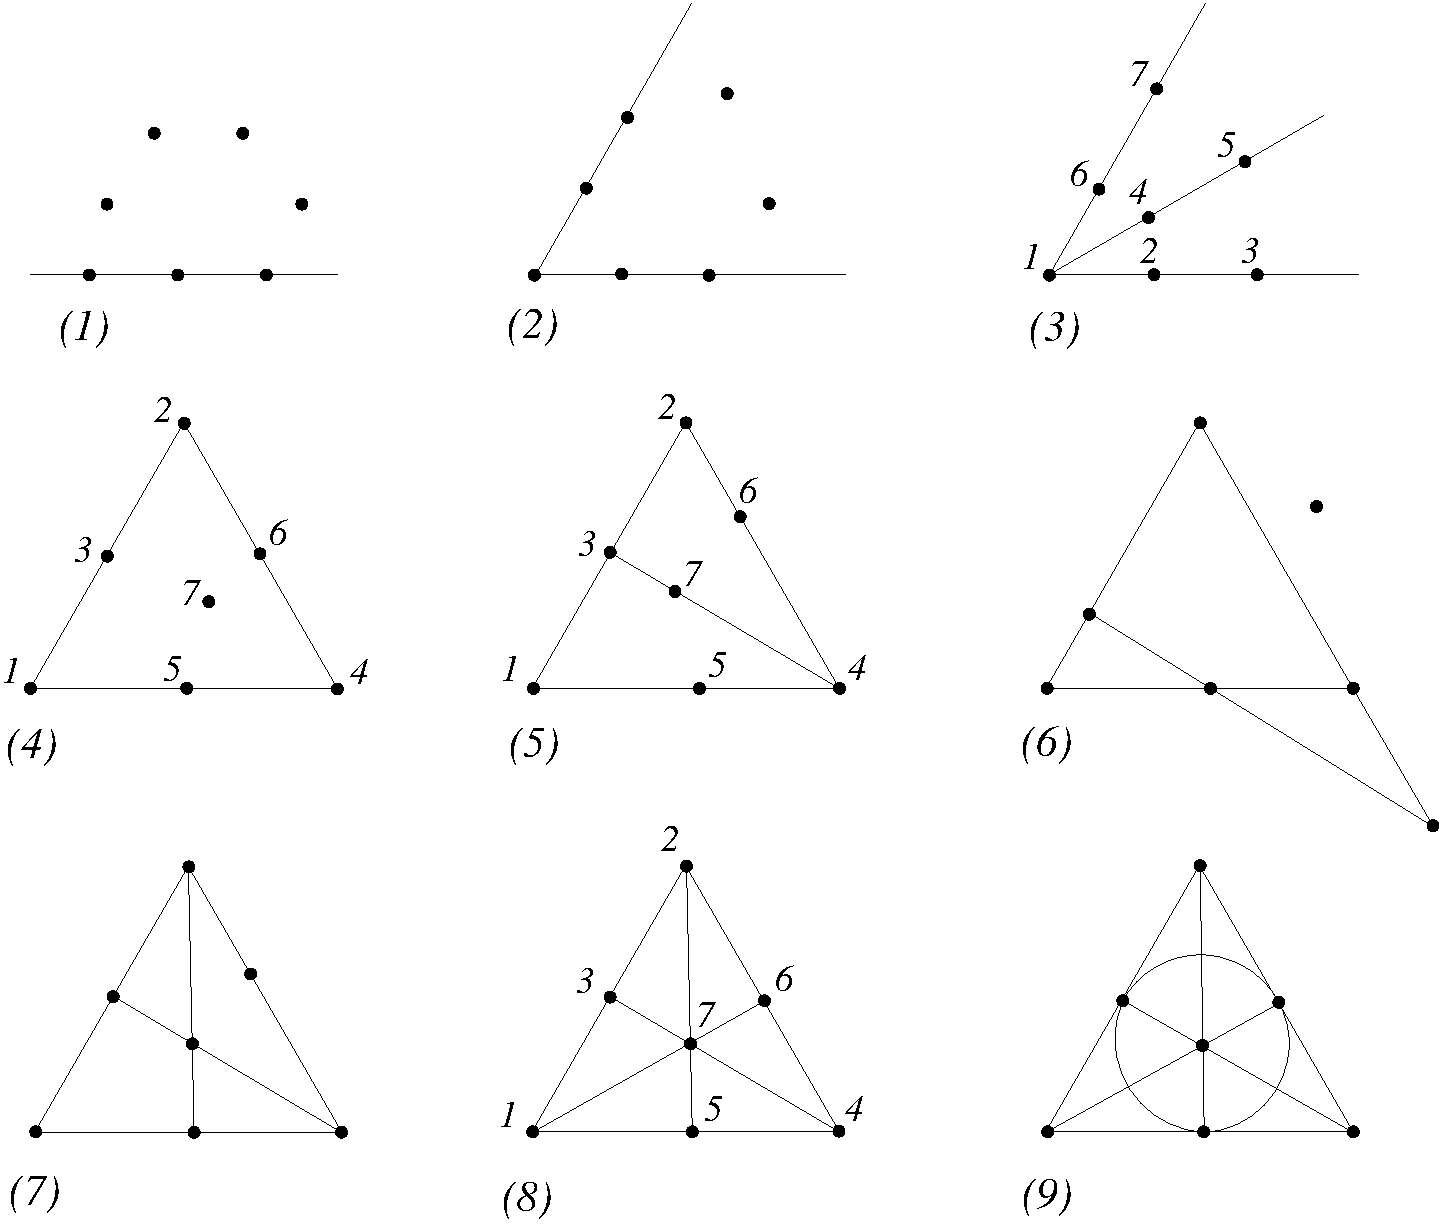
\includegraphics[height=9cm]{noveConfB.pdf}
\caption{Possible collinearities of $7$ points
\label{collin}}
\end{figure}


%%%% file per questa proposizione:
%%%% d1d1NO.sage
\begin{lemma} If we have $7$ eigenpoint of a cubic curve in configuration
  $(3)$, then necessarily $\delta_2(P_1, P_2, P_3, P_4, P_5)=0$, but
  configuration $(3)$ cannot be realized by the conditions
  $\delta_1(P_1, P_2, P_4) = 0$ and
  $\delta_1(P_1, P_2, P_6)=0$.
\end{lemma}
\begin{proof}
As we know from proposition~\ref{propX}, configuration $(3)$ can be realized
if the condition $\delta_2(P_1, P_2, P_3, P_4, P_5) = 0$ holds.
Suppose now that we have
$\delta_1(P_1, P_2, P_4) = 0$ and  $\delta_1(P_1, P_2, P_6)=0$. These
two equations give a linear system in the coordinates of $P_2$ that can
be easily solved. The associated matrix has rank $2$ unless
$\scl{P_1}{P_1}=0$ (DA FARE@@@@). If $\scl{P_1}{P_1} \not = 0$,
the solution of the system gives:
\[
(A_2, B_2, C_2) = \scl{P_1}{P_1} \cdot det([P_1, P_4, P_6])\cdot P_1
\]
which says that, as projective points, $P_1$ and $P_2$ coincide and this is
not possible. 
\end{proof}

%%%%% file per questa proposizione:
%%%%% arcibaldo3.sage
\begin{prop}
Let $P_i(A_i, B_i, C_i)$, for $i=1, 2, 4$
be three distinct points in the plane not aligned and let
$P_3$ be a point on the line $P_1+P_2$, $P_5$ a point on the line
$P_1+P_4$ and $P_6$ a point on the line $P_2+P_4$ (i.e.\ assume that
the points are in the configuration $(4)$ of figure~\ref{collin}).
If these points are eigenpoints of a cubic curve, then
necessarily the point $P_7$ (the seventh eigenpoint) is on the intersection
of the lines $P_1+P_6$, $P_3+P_4$ and $P_2+P_5$, i.e.\ the points are in
configuration (8).
\label{prp4}
\end{prop}
\begin{proof}
  Let $(A_i, B_i, C_i)$ be the coordinates of $P_i$ for $i=1, 2, 4$ and let
  $P_3 = u_1P_1+u_2P_2$, $P_5 = v_1P_1+v_2P_4$ and $P_6 = w_1P_2+w_2P_4$.
  If configuration $(4)$ is possible, then proposition~\ref{freccia} gives that
  $\delta_1(P_1, P_2, P_4)$,  $\delta_1(P_4, P_1, P_2)$ and
  $\delta_1(P_2, P_1, P_4)$ must be zero. We define therefore the ideal
  generated by them and, in order to exclude degenerate cases,
  we saturate it w.r.t.\ the three ideals of the
  coordinates of $P_1$, $P_2$ and $P_4$ and with the polynomial
  given by $\det([P_1, P_2, P_4])$. The ideal we obtain gives that:
  \[
  \scl{P_1}{P_2}=0, \quad \scl{P_1}{P_4}=0, \quad
  \scl{P_2}{P_4}=0
  \]
    {From} the definition of $\delta_2$ given in proposition~\ref{propFrc}
    we get that
\[
\delta_2(P_1, P_3, P_2, P_5, P_4) = 0, \quad
\delta_2(P_2, P_3, P_1, P_6, P_4) = 0, \quad
\delta_2(P_4, P_5, P_1, P_6, P_2) = 0
\]
hence, from proposition~\ref{propX}, we have that $P_7$ lies on the lines
$P_1+P_6$, $P_2+P_5$ and $P_3+P_4$. In conclusion, configuration $(4)$ of
figure~\ref{collin} cannot be realized since gives configuration $(8)$.
\end{proof}



%%%% file per questa proposizione:
%%%% arcibaldo2.sage
\begin{prop}
  Let $P_1, \dots, P_4$ be four points in the plane,
  let $P_5$ be the intersection point of the lines $P_1+P_4$
  and $P_2+P_3$ and let $P_6$ be the intersection point of the lines
  $P_1+P_2$ and $P_3+P_4$ (i.e.\ assume that the points are in configuration
  $(6)$ of figure~\ref{collin}). Then this configuration cannot be realized by
  the eigenpoints of a cubic curve. 
\end{prop}
\begin{proof}
  If configuration $(6)$ can be realized by eigenpoints,
  from proposition~\ref{},
  it must hold:
  \[
  \begin{array}{lll}
\delta_1(P_1, P_2, P_5)=0,&\delta_1(P_2, P_1, P_5)=0,&\delta_1(P_6, P_2, P_4)=0,\\ 
\delta_1(P_4, P_1, P_6)=0,& \delta_1(P_5, P_1, P_3)=0,&\delta_1(P_3, P_5, P_4)=0
\end{array}
  \]
  We construct therefore the ideal generated by the above polynomial and we
  saturate it w.r.t.\ the condition that there are no collinearities among three
  points chosen within the points $P_1, \dots, P_4$ and the condition that
  the couples $(P_1, P_4)$ and $(P_3, P_4)$ are distinct (in order to speed up the
  computations, it is convenient to first factorize the six polynomials, erase the
  useless factors and then saturate the remaining ideal).
  After all the above saturations, we get the ideal $\langle 1\rangle$, which
  shows that the configuration (6) is not realizable by eigenpoints.
\end{proof}


%%%%%% i conti per questo caso sono nel file
%%%%%% arcibaldo4.sage
\begin{prop}
  Configuration $(5)$ can be realized. Moreover, we can give an explicit
  description
  of the family of all the points $P_1, \dots, P_6$ of the plane in
  configuration $(5)$ which
  are eigenpoints and they are given by
  \[
  \begin{array}{rcl}
    P_4 &=& P_1 \wedge P_2\\
    U_2 &=& s_{12}^2v_2w_1 + s_{11}s_{22}v_2w_1 + 2s_{11}s_{24}v_2w_2
    - 2s_{11}s_{25}w_2\\    
    U_1 &=& 2s_{12}s_{22}v_2w_1 + s_{14}s_{22}v_2w_2 + s_{12}s_{24}v_2w_2
    - s_{15}s_{22}w_2 - s_{12}s_{25}w_2\\
    P_3 &=& U_2P_1 - U_1P_2\\
    P_5 &=& v_1P_1+v_2P_4 \\
    P_6 &=& w_1P_2+w_2P_4
  \end{array}
  \]
  (where $P_1, P_2, v_1, v_2, w_1, w_2$ can be chosen in an arbitrary way). 
\end{prop}
\begin{proof}
  In order to have configuration $(5)$, we have:
  $P_3 = u_1P_1+u_2P_2$, $P_5 = v_1P_1+v_2P_4$, $P_6 = w_1P_2+w_2P_4$ and
  the equations $\delta_1(P_1, P_2, P_4) = 0$, $\delta_1(P_2, P_1, P_4) = 0$,
  $\delta_2(P_4, P_5, P_1, P_2, P_6) = 0$ that have to be satisfied.
  The corresponding ideal (after
  saturation w.r.t.\ the polynomial $\det([P_1, P_2, P_4])$, is
  the ideal $(s_{14}, s_{24})$, therefore $P_4$ must be the point
  $P_1 \wedge P_2$ and $P_5$ and $P_6$ are consequently modified.
  We have to see under which conditions the $18\times 10$ matrix
  whose rows are $\phi_i(P_j)$ for $i=1, 2, 3$, $j=1, \dots, 6$ has
  rank less than $10$. Several order ten minors are already zero, as
  a consequence of the conditions $\delta_1$ and $\delta_2$ imposed on
  the points.
  Then we
  compute the determinant of the order ten matrix whose rows are
  $\phi_i(P_j)$ for $i=1, 2$ and
  $j = 1, \dots, 4$, $\phi_1(P_5)$ and $(t_1, \dots, t_{10})$.
  Successively we substitute
  to $(t_1, \dots, t_{10})$ the three vectors $\phi_k(P_6)$ for $k=1, 2, 3$
  and we get, respectively:
  \[(s_{12}C_2-s_{22}C_1)(s_{11}s_{22}-s_{12}^2)\cdot F, \quad
  (s_{12}B_2-s_{22}B_1)(s_{11}s_{22}-s_{12}^2)\cdot F,\quad
  (s_{12}A_2-s_{22}A_1)(s_{11}s_{22}-s_{12}^2)\cdot F
  \]
  where $F = U_1u_1+U_2u_2$.
  If $s_{12}A_2-s_{22}A_1=0$, $s_{12}B_2-s_{22}B_1=0$, $s_{12}C_2-s_{22}C_1=0$,
  then this is implies $s_{22}=0$, $s_{12} = 0$ @@da fare@@. In the general case
  we choose $u_1 = U_2$ and $u_2 = -U_1$, so $P_3=U_2P_1 - U_1P_2$;
  the matrix whose rows are $\phi(P_i)$ for $i=1, \dots, 6$ has rank
  less then $10$, so the six points are eigenpoints.
  \end{proof}


%%%% conti per questa prop: arcibaldo6.sage
In proposition~\ref{prp4} we sow that configuration $(4)$ implies
configuration $(8)$ which is therefore realizable.
Now we can be more precise:

\begin{prop} Configuration $(8)$ can be realized. Moreover, we can give an
  explicit description of the family of all points $P_1, \dots, P_7$ of
  the plane in configuration $(8)$ which are eigenpoints and they are given
  by
  \[
  \begin{array}{rcl}
    P_4 &=& (P_1\wedge P_2)\scl{P_1}{P_3}\scl{P_2}{P_3}-
    \scl{P_1}{P_2}(P_1 \wedge P_3) \scl{P_2}{P_3}+
    \scl{P_1}{P_2}\scl{P_1}{P_3}(P_2 \wedge P_3)\\
    P_5 &=& (P_1+P_2) \cap (P_3+P_4) \\
    P_6 &=& (P_1+P_4) \cap (P_2+P_3) \\
    P_7 &=& (P_1+P_3) \cap (P_2+P_4) 
  \end{array}
  \]
  (where $P_1, P_2, P_3$ can be chosen in an arbitrary way). 
\end{prop}
\begin{proof}
Let $P_i(A_i, B_i, C_i)$, for $i=1, \dots, 4$
be four generic points in the plane and $P_5$
be the point of intersection of $P_1+P_2$ and $P_3+P_4$,
$P_6$ be the point of intersection of $P_1+P_4$ and $P_2+P_3$,
$P_7$ be the point of intersection of $P_1+P_3$ and $P_2+P_4$.
In order to obtain configuration $(8)$ it must hold:
\[
e_1 = \delta_1(P_5, P_1, P_4) = 0, \quad
e_2 = \delta_1(P_6, P_1, P_2) = 0, \quad
e_3 = \delta_1(P_7, P_1, P_2) = 0.
\]
The computation gives:
\[
\begin{array}{rcl}
e_1 & =& -\det([P_1, P_3, P_4]) \det([P_1, P_2, P_4])
\left(\scl{P_1\wedge P_2}{P_3 \wedge P_4} \right)\\
e_2 & =& \det([P_1, P_2, P_4]) \det([P_1, P_2, P_3])
\left(\scl{P_1\wedge P_4}{P_2 \wedge P_3} \right)\\
e_3 & =& \det([P_2, P_3, P_4]) \det([P_1, P_3, P_4])
\left(\scl{P_1\wedge P_3}{P_2 \wedge P_4} \right)
\end{array}
\]
Since there are no three collinear points among $P_1, P_2, P_3, P_4$,
we can redefine $e_1, e_2, e_3$ by:
\[
\begin{array}{rcl}
  e_1 & = & -\left(\scl{P_1\wedge P_2}{P_3 \wedge P_4} \right)\\
  e_2 & = & \left(\scl{P_1\wedge P_4}{P_2 \wedge P_3} \right)\\
  e_3 & = & \left(\scl{P_1\wedge P_3}{P_2 \wedge P_4} \right)
\end{array}
\]
and we see that $e_1-e_2+e_3 = 0$ so we have to solve the equations
$e_1=e_2=0$.
The system $e_1 = 0, e_2 = 0$ is linear in $A_4, B_4, C_4$. The 
matrix associated to the system has rank $2$ unless one of the following
three conditions is satisfied:
\[
\scl{P_1}{P_2} = \scl{P_1}{P_3} = 0, \mbox{ or }
\scl{P_2}{P_3} = \scl{P_1}{P_3} = 0, \mbox{ or }
\scl{P_1}{P_2} = \scl{P_2}{P_3} = 0
\]
Condizioni da studiare a parete @@
So, when the matrix has rank $2$ we can determine its solution
and it is possible to see that $P_4$ is given by the expression above.
Consequentely we define $P_5, P_6, P_7$. Then it holds:
\[
\begin{array}{ll}
  \delta_2(P_1, P_2, P_5, P_3, P_7) = 0 & 
\delta_2(P_2, P_1, P_5, P_7, P_4) = 0 \\
\delta_2(P_4, P_1, P_6, P_2, P_7) = 0 & 
\delta_2(P_1, P_7, P_3, P_4, P_6) = 0
\end{array}
\]
and these conditions allow to find that the rank of the $21\times 10$
matrix whose rows are $\phi_i(P_j)$ ($i = 1, 2, 3$, $j = 1, \dots, 7$)
has rank less than $10$, hence the points are eigenpoints. 
\end{proof}


\begin{example}
  Take three random points, like
  $P_1, P_2, P_3 = (2, -1, 5), (3, 2, 1), (-1, 4, 3)$
  Then $P_4$, defined by the above formula, is $(19, 17, 21)$
  and, consequetly, $P_5, P_6, P_7 = (195, 88, 143), (4, 5, 3), (55, 158, 429)$
  The matrix of these points has rank $9$, the cubic curve whose
  eigenpoints are $P_1, \dots, P_7$ in configuration $(8)$ has equation:
  \[
1427x^3 + 2409x^2y + 429xy^2 + 1553y^3 + 1617x^2z - 2562xyz + 3003y^2z + 1113xz^2 + 105yz^2 + 2219z^3
  \]
\end{example}
\begin{prop} Configuration $(9)$ is not realizable.
\end{prop}
\begin{proof}
  The collinearities of the points give the Fano plane, which is not
  realizable in characteristic zero.
\end{proof}

\section{Particular Cases}
Concerning proposition~\ref{prototipo}:

All triplets $P_1, P_2, P_3$ of points such that are collinear and
\[\scl{P_1}{P_1} = 0, \scl{P_1}{P_2} = 0, \scl{P_1}{P_3} = 0
\]
are given by:
\begin{eqnarray*}
P_1 &=& (i(l^2-n^2), 2iln, l^2+n^2) \\
P_2 &=& (-C_2(l^2+n^2) - 2iB_2ln, B_2i(l^2-n^2), C_2i(l^2-n^2))\\
P_3 &=& u_1P_1+u_2P_2
\end{eqnarray*}
where $l, n, B_2, C_2$ are arbitrary elements of $K$ (and $i=\sqrt{-1}$).

\bigskip
Points $P_1, P_2, P_3, P_4, P_5$ such that 
$\scl{P_1}{P_1}\scl{P_2}{P_2}-\scl{P_1}{P_2}^2 = 0$ and such that also
$\delta_1(P_1, P_2, P_4)=0$.

The coordinates are the following:
\begin{eqnarray*}
  P_1 &=& (l^2+m^2-n^2, 2ln, 2mn)\\
  P_2 &=& (-B_2l^2 + iC_2l^2 -2iB_2lm-2C_2lm + B_2m^2-iC_2m^2 + B_2n^2 + iC_2n^2,\\
  & & -2B_2ln -2iB_2mn, -2C_2ln -2iC_2mn)\\
  P_3 &=& u_1P_1+u_2P_2\\
  P_4 &=& (-B_4l^2 + iC_4l^2 -2iB_4lm-2C_4lm + B_4m^2 -iC_4m^2+B_4n^2 + iC_4n^2,\\
  & & -2B_4ln -2iB_4mn, -2C_4ln -2iC_4mn)\\
  P_5 &=& v_1P_1+v_2P_4
\end{eqnarray*}
It is immediate to see that then also $\delta_2(P_1, P_2, P_3, P_4, P_5) = 0$

Sembra che in questo caso la cubica sia riducibile. Conti da completare.
Pare che la matrice $M$ in questo caso ha rango $6$. Conti da completare.
@@@
\end{document}









\begin{prop}
Let $P_i(A_i, B_i, C_i)$, for $i=1, \dots, 4$
be four generic points in the plane and $P_5$
be the point of intersection of $P_1+P_4$ and $P_2+P_3$,
let  $P_6$ be the point of intersection of $P_1+P_2$
and $P_3+P_4$. If we assume that these points are eigenpoints of a cubic,
the lines $P_1+P_3$ and $P_2+P_4$ meet in a point $P_7$ which is an
eigenpoint.
\end{prop}
\begin{proof}
  Under our hypotheses, $P_5$, $P_6$ and $P_7$ cannot be aligned. 
  The points $P_6, P_1, P_2$ and $P_6, P_3, P_4$ are collinear, hence, by
  proposition~\ref{freccia}, $\delta_1(P_6, P_1, P_3) = 0$ or
  $\delta_2(P_6, P_1, P_2, P_3, P_4) = 0$. But this last condition,
  by proposition~\ref{propX}, implies that $P_5$, $P_6$ and $P_7$
  are aligned, which is not possible hence, necessarily,
  $\delta_1(P_6, P_1, P_4) = 0$. Similarly, $\delta_1(P_5, P_1, P_2) = 0$.
  Consider the following polynomials:
\begin{eqnarray*}
  \delta_1(P_5) & = & \delta_1(P_5, P_1, P_2) \\
  \delta_1(P_6) & = & \delta_1(P_6, P_1, P_4) \\
  \delta_1(P_7) & = & \delta_1(P_7, P_2, P_3) 
\end{eqnarray*}
It holds:
\begin{eqnarray*}
  \delta_1(P_5) & = & \det([P_1, P_2, P_3]) \cdot \det([P_1, P_2, P_4])\cdot\\
  & &   \left(\scl{P_1}{P_2}\scl{P_3}{P_4}-\scl{P_1}{P_3}\scl{P_2}{P_4}\right)
\end{eqnarray*}
and similar formulas are obtained for $\delta_1(P_6)$ and $\delta_1(P_7)$.
Since we assume that $P_1, P_2, P_3$ and $P_1, P_2, P_4$ are not collinear,
\[
\delta_1(P_5)=0 \mbox{ if and only if }
\scl{P_1}{P_2}\scl{P_3}{P_4}-\scl{P_1}{P_3}\scl{P_2}{P_4}=0
\]
Similarly, 
\[
\delta_1(P_6)=0 \mbox{ if and only if }
\scl{P_1}{P_4}\scl{P_2}{P_3}-\scl{P_1}{P_3}\scl{P_2}{P_4}=0
\]
and
\[
\delta_1(P_7)=0 \mbox{ if and only if }
\scl{P_1}{P_2}\scl{P_3}{P_4}-\scl{P_1}{P_4}\scl{P_2}{P_3}=0
\]
and we see that $\delta_1(P_7) = \delta_1(P_5) - \delta_1(P_6)$. This show
that, if $\delta_1(P_5) = 0$ and $\delta_1(P_6) = 0$, then $\delta_1(P_7) = 0$,
therefore there exists a cubic which has the eigenpoints
$P_7, P_1, P_2, P_3, P_4$ but, for the genericity of the points
$P_1, \dots, P_4$ (@@ sara' giusto? va un po' sistemato) this cubic is unique
and hence is the cubic which has $P_1, \dots, P_6$ as eigenpoints. 
\end{proof}

\begin{cor}
Among the $7$ eigenpoints of a cubic curve,
configuration $(6)$ and $(7)$ are not possible.
\end{cor}

%\noindent
%\textbf{Prop.} Configuration $(4)$ is not realizable.
%% vedi file: configurationN4.sage



We consider now eigenpoints $P_1, \dots, P_6$ which have (at least)
the configuration $(4)$ of figure~\ref{collin}.

To the points $P_i$ we give coordiantes 
$(A_i, B_i, C_i)$ (for $i = 1, 2, 4$) and we set
$P_3 = u_1P_1+u_2P_2$,
$P_5 = v_1P_1+v_2P_4$ and $P_6 = w_1P_2+w_2P_4$, 
In particular, if configuration $(4)$ is satisfied, we have that
\[
\left\{
\begin{array}{rcl}
  \delta_1(P_1, P_2, P_4) &=&  0\\
  \delta_1(P_1, P_2, P_4) &=&  0\\  
\end{array}
\right.
\]
This is a homogeneous linear system in $A_4, B_4, C_4$, so we can
construct the associated matrix $M$. In order to see the rank of
$M$ we compute its maximal minors and they are:
\[
l(B_1A_2-B_2A_1),\quad l(C_1A_2-C_2A_1) \quad l(B_2C_1-B_1C_2)
\]
where
\begin{eqnarray*}
  l &=& \scl{P_1}{P_1}\scl{P_2}{P_2}-\scl{P_1}{P_2}^2\\
  & = & |P_1 \wedge P_2 |^2
\end{eqnarray*}
Since we assume that $P_1$ and $P_2$, as projective points, are distinct,
then $P_1 \wedge P_2 \not = 0$ and therefore $M$ is of maximal rank.
@@@ questo su R, pero' c'e' ancora da considerare il caso in C. 

We can solve the linear system (with Kramer) and we find that $P_4$, as
a projective point, is given by:
\[
P_4 = P_1 \wedge P_2
\]
Hence we re-define $P_4$ with this condition and $P_5$ and $P_6$ 
consequentely. With these new coordinates of the points, it is
immediate to verify that:
$\delta_2(P_4, P_1, P_5, P_2, P_6) = 0$, therefore, as a consequence of @@,
we have:

\begin{prop}
If a configuration of six eigenpoints $P_1, \dots, P_6$ with
at least the collinearities $(P_1, P_2, P_3)$, $(P_1, P_4, P_5)$ and
$(P_2, P_4, P_6)$ exists, then the 7th eigenpoint $P_7$ is collinear with
$P_3$ and $P_4$.
\end{prop}

As a consequence we have:
\begin{prop} Configuration $(4)$ and $(6)$ cannot be realized by
  eigenpoints.
  \end{prop}

Concerning configuration $(5)$, the above computation shows that
it could be obtained,
provided $P_1, \dots, P_6$ are eigenpoints. The first
problem is, therefore, to see when $P_1, \dots, P_6$ are eigenpoints.

We consider the following two square matrices of order $10$:
$M_1$ whose rows are:
$\phi_1(P_i), \phi_2(P_i) $ for $i = 1, 2, 3, 4$ and the two other rows
are $\phi_1(P_5)$ and $\phi_1(P_6)$ and $M_2$, whose rows are:
$\phi_1(P_i), \phi_2(P_i) $ for $i = 1, 2, 3, 4$ plus the rows
$\phi_1(P_5)$ and $\phi_2(P_6)$.

Since the order of the matrix $M$ whose rows are $\phi_j(P_i)$ for
$j = 1, 2, 3$ and $i = 1, \dots 6$ must be $9$, the 
determinant of these two matrices must be zero. Their computation
gives that they have a common factor, which is a polynomial
of degree one in $u_1, u_2, v_1, v_2, w_1, w_2$. Therefore, if we fix
$v_1, v_2, w_1, w_2$, we can solve the homogeneous linear equation in
$u_1$ and $u_2$, obtaining a solution which annihilates the two
above determinants. With this condition on $u_1$ and $u_2$ we find a
point $P_3$ such that $P_1, \dots, P_6$ are eigenpoints of a cubic $c$
and the $7$ eigenpints of $c$ are (in general) in
configuration $(5)$. In particular we have:

\begin{prop} Cubics with $7$ eigenpoints in configuration $(5)$ exist
and are parametrized by (((an open subset of))) of
$\mathbb{P}^2 \times \mathbb{P}^2 \times \mathbb{P}^1 \times \mathbb{P}^1$.
\end{prop}
Here is an example: take two points:
\[
P_1 = (-2, -3/2, 1) \ \mbox{ and } \ 
P_2 = (-1/7, 11/7, 1).
\]
Then $P_4 = P_1\wedge P_2 = (43/47, -26/47, 1)$.
Then we consider $P_5 = 2P_1-13P_4$, $P_6 = -5P_2+17P_4$ and
$P_3 = u_1P_1+u_2P_2$. We compute the $18\times 10$ matrix $M$
given by $\phi_j(P_i)$ and it is
of rank $9$ if $51230u_1 + 26199u_2=0$. We obtain the cubic curve of
equation:
\[
\begin{array}{l}
  9577808741x^3 + 22652178147x^2y + 14272951368xy^2 + \\
  6238979384y^3 - 14246840901x^2z - 25064993838xyz -\\
  2883255336y^2z + 5566105107xz^2 + 10194620043yz^2 - 12662243z^3
\end{array}
\]
with the following $7$ eigenponts:
\[
\begin{array}{l}
(-2, -3/2, 1),\quad (-1/7, 11/7, 1), \quad (-6001/15808, 484933/411008, 1), \\
  (43/47, -26/47, 1), \quad  (551/615, -344/615, 1),
  \quad (184/191, -497/764, 1)\\
  (4017587443/4085422235, -2634690152/4085422235, 1) 
\end{array}
\]
which are aligned according to configuration $(5)$.

\begin{prop}
  Configuration $(3)$ can be obtained (with condition $\delta_2$) but
  cannot be optained with two conditions $\delta_1$. (@@ a parte il caso
  $\scl{P_1}{P_1}=0$ ??).
\end{prop}
\begin{proof}
  We define the following four points with generic coordinates:
  $P_i = (A_i, B_i, C_i)$ for $i = 1, 2, 4, 6$. Then we compute
  $e_1 = \delta_1(P_1, P_2, P_4)$ and $e_2 = \delta_1(P_1, P_2, P_6)$. 
  We see that $e_1$ and $e_2$ are linear in $A_2, B_2, C_2$, so we construct
  the matrix of the linear system $e_1 = 0, e_2 = 0$ with respect to these
  variables. We get a matrix whose maximal minors are:
  \[
  C_1 \scl{P_1}{P_1} \Delta, \quad
  -B_1 \scl{P_1}{P_1} \Delta, \quad
  A_1 \scl{P_1}{P_1}  \Delta
  \]
  where $\Delta = \det([P_1, P_4, P_6])$.
  From this we get that the solution of the system  (if
  $\scl{P_1}{P_1} \not = 0$) gives that $P_2$ coincides, as projective
  point, with $P_1$, and this is not possible. 
\end{proof}

We come now to the configuration $(8)$ of figure @@@.
In order to construct points satisfying the given collinearities,
we define in an arbitray way the points $P_i$ for $i = 1, 2, 4, 7$
and consequentely we compute the point $P_3$ as the intersection
of the lines $P_1+P_2$ and the line $P_4+P_7$, the point $P_5$ as
$(P_2+P_7)\cap (P_1+P_4)$ and $P_6$ as $(P_1+P_7)\cap (P_2+P_4)$.
In this way we have the coordinates of all the $7$ points in terms of
the coordinates of $P_1, P_2, P_4, P_7$. 
According to the
labels of the points in the figure, we see that, if we set:
\begin{eqnarray*}
  e_1 & = & \delta_1(P_3, P_2, P_4)  \\
  e_2 & = & \delta_1(P_5, P_2, P_4) \\
  e_3 & = & \delta_1(P_6, P_1, P_2)
\end{eqnarray*}
at least the conditions $e_1=0, e_2=0, e_3 = 0$ have to be satisfied.
The computation of $e_1$ gives:
\[
e_1 = \det([P_2,P_4,P_7])\det([P_1, P_2, P_4])
\left(\scl{P_1}{P_7}\scl{P_2}{P_4}-\scl{P_1}{P_4}\scl{P_2}{P_7} \right)
\]
Similar formulas hold for $e_2$ and $e_3$.
Since the two determinants must be different from zero, we can erase them
and re-define $e_1, e_2, e_3$ and we get:
\begin{eqnarray*}
  e_1 & = &
  \scl{P_1}{P_7}\scl{P_2}{P_4}-\scl{P_1}{P_4}\scl{P_2}{P_7} \\
  e_2 & = &
  \scl{P_1}{P_7}\scl{P_2}{P_4}-\scl{P_1}{P_2}\scl{P_4}{P_7} \\
  e_3 & = &
  \scl{P_1}{P_2}\scl{P_4}{P_7}-\scl{P_1}{P_4}\scl{P_2}{P_7} \\  
\end{eqnarray*}
In particular, we see that $e_3 = e_1 - e_2$, so it is not necessary
to consider the equation $e_3=0$. Concerning the other two equations
$e_1 = 0$ and $e_2 = 0$, they are both linear in $A_1, B_1, C_1$ threfore
we can solve the linear system and we get the following solution for
$A_1, B_1, C_1$:
\begin{eqnarray*}
A_1 &=&s27s47C2B4 - s27s47B2C4 - s24s47C2B7 + s24s27C4B7 + s24s47B2C7 - s24s27B4C7\\
B_1 &=&-s27s47C2A4 + s27s47A2C4 + s24s47C2A7 - s24s27C4A7 - s24s47A2C7 + s24s27A4C7\\
C_1 &=&s27s47B2A4 - s27s47A2B4 - s24s47B2A7 + s24s27B4A7 + s24s47A2B7 - s24s27A4B7
\end{eqnarray*}
(where $sij = \scl{P_i}{P_j}$).

This solution, after some manipulations, gives:
\[
P_1 = (P_2 \wedge P_4) \scl{P_2}{P_7}\scl{P_4}{P_7}-
\scl{P_2}{P_4} (P_2 \wedge P_7) \scl{P_4}{P_7}+
 \scl{P_2}{P_4}\scl{P_2}{P_7} (P_4 \wedge P_7)
\]

According to the collinearities of the points
the conditions $\delta_2(P_1, P_2, P_3, P_4, P_5)=0$,
$\delta_2(P_2, P_1, P_3, P_4, P_6)=0$
and $\delta_2(P_4, P_1, P_5, P_2, P_6)=0$
should be satisfied but these conditions do not give other equations to
solve, since, if we substitute
the values of $A_1, B_1, C_1$ into these three polynomials
we get zero in each of the three cases. 
Hence the $7$ points are eigenpoints and the configuration
$(8)$ is obtained. Therefore we have:

\begin{prop}
  Condition $(8)$ can be realized. Cubics with eigenpoints in that
  configuration are parametrized by (((an open subset of)))
  $\mathbb{P}^2\times \mathbb{P}^2\times \mathbb{P}^2$.
\end{prop}


An example:\\
we define three points (in a random way):
$P_2 = (1, -3, 11)$, $P_4 = (-3, 2, -5)$ and
$P_7 = (6, -11, 2)$. Consequentely, we compute 
$P_1 = (1171, 204, 659)$. Then the remaining points (obtained as intersection
of lines passing through the given points) are:
$P_3 = (305, -89, 639)$, $P_5 = (1285, -2826, 4727)$, $P_6 = (8, -3, 4)$.

The cubic curve is:
\[
\begin{array}{l}
  9143x^3 - 696x^2y + 14064xy^2 - 8872y^3 + 10257x^2z + 6816xyz + 5712y^2z +\\
  1797xz^2 - 4152yz^2 + 10427z^3
\end{array}
\]
\begin{prop} Configuration $(9)$ is not realizable.
\end{prop}
\begin{proof}
  The collinearities of the points give the Fano plane, which is not
  realizable in characteristic zero.
\end{proof}



\bigskip
------------------------

%%%%
%%%% questi conti stanno sul file line_r3.sage
%%%%

We come back to the proof of Proposition~\ref{prop2}.
It is possible to see that the equation of the line $r_3$ can be written in
the following way.

Let
\begin{eqnarray*}
V_{11} & = & (\scl{P_1}{P_2}\scl{P_1}{P_4} - \scl{P_1}{P_1}\scl{P_2}{P_4})  (-\scl{P_1}{P_4}^2\scl{P_2}{P_2} + \scl{P_1}{P_2}^2\scl{P_4}{P_4})\\
V_{12} & = & (\scl{P_1}{P_4}\scl{P_2}{P_4} -\scl{P_1}{P_2}\scl{P_4}{P_4})  (\scl{P_1}{P_4}^2\scl{P_2}{P_2} - \scl{P_1}{P_2}^2\scl{P_4}{P_4})\\
V_{21} & = & \scl{P_1}{P_1}  (\scl{P_1}{P_4}\scl{P_2}{P_2} - \scl{P_1}{P_2}\scl{P_2}{P_4})  (\scl{P_1}{P_4}^2 - \scl{P_1}{P_1}\scl{P_4}{P_4})\\
V_{22} & = & (\scl{P_1}{P_4}^2 - \scl{P_1}{P_1}\scl{P_4}{P_4})  (\scl{P_1}{P_4}^2\scl{P_2}{P_2} - 2\scl{P_1}{P_2}\scl{P_1}{P_4}\scl{P_2}{P_4} + \scl{P_1}{P_2}^2\scl{P_4}{P_4})\\
V_{31} & = & \scl{P_1}{P_1}  (\scl{P_1}{P_4}\scl{P_2}{P_4} - \scl{P_1}{P_2}\scl{P_4}{P_4})  (\scl{P_1}{P_2}^2 - \scl{P_1}{P_1}\scl{P_2}{P_2})\\
V_{32} & = & -\scl{P_1}{P_2}\scl{P_1}{P_4}^3\scl{P_2}{P_2} + 2\scl{P_1}{P_2}^2\scl{P_1}{P_4}^2\scl{P_2}{P_4} - \scl{P_1}{P_1}\scl{P_1}{P_4}^2\scl{P_2}{P_2}\scl{P_2}{P_4}
- \scl{P_1}{P_2}^3\scl{P_1}{P_4}\scl{P_4}{P_4} + 2\scl{P_1}{P_1}\scl{P_1}{P_2}\scl{P_1}{P_4}\scl{P_2}{P_2}\scl{P_4}{P_4} - \scl{P_1}{P_1}\scl{P_1}{P_2}^2\scl{P_2}{P_4}\scl{P_4}{P_4}
\end{eqnarray*}
then the equation of the line $r_3$ is:
\[
\scl{\scl{(x, y, z)}{(P_1, P_2, P_4)}}{(V_{11}v_1+V_{12}v_2,V_{21}v_1+V_{22}v_2,V_{31}v_1+V_{32}v_2)}
\]
\end{document}
